%!TEX root = ../../../../build/bioseqdb_presentation1/_prebuild/main.tex
% type: technicalslides
% title: BioseqDB - entry presentation 1
% created: 2025-12-15


% START


\newcommand{\foo}{\color{black}\makebox[0pt]{\textbullet}\hskip-0.5pt\vrule width 1pt\hspace{\labelsep}}
\newenvironment{itemizesmall}{\itemize\addtolength{\itemsep}{-\baselineskip}}{\enditemize}

{
\hypersetup{linkcolor=white}
\setbeamertemplate{background} 
{
    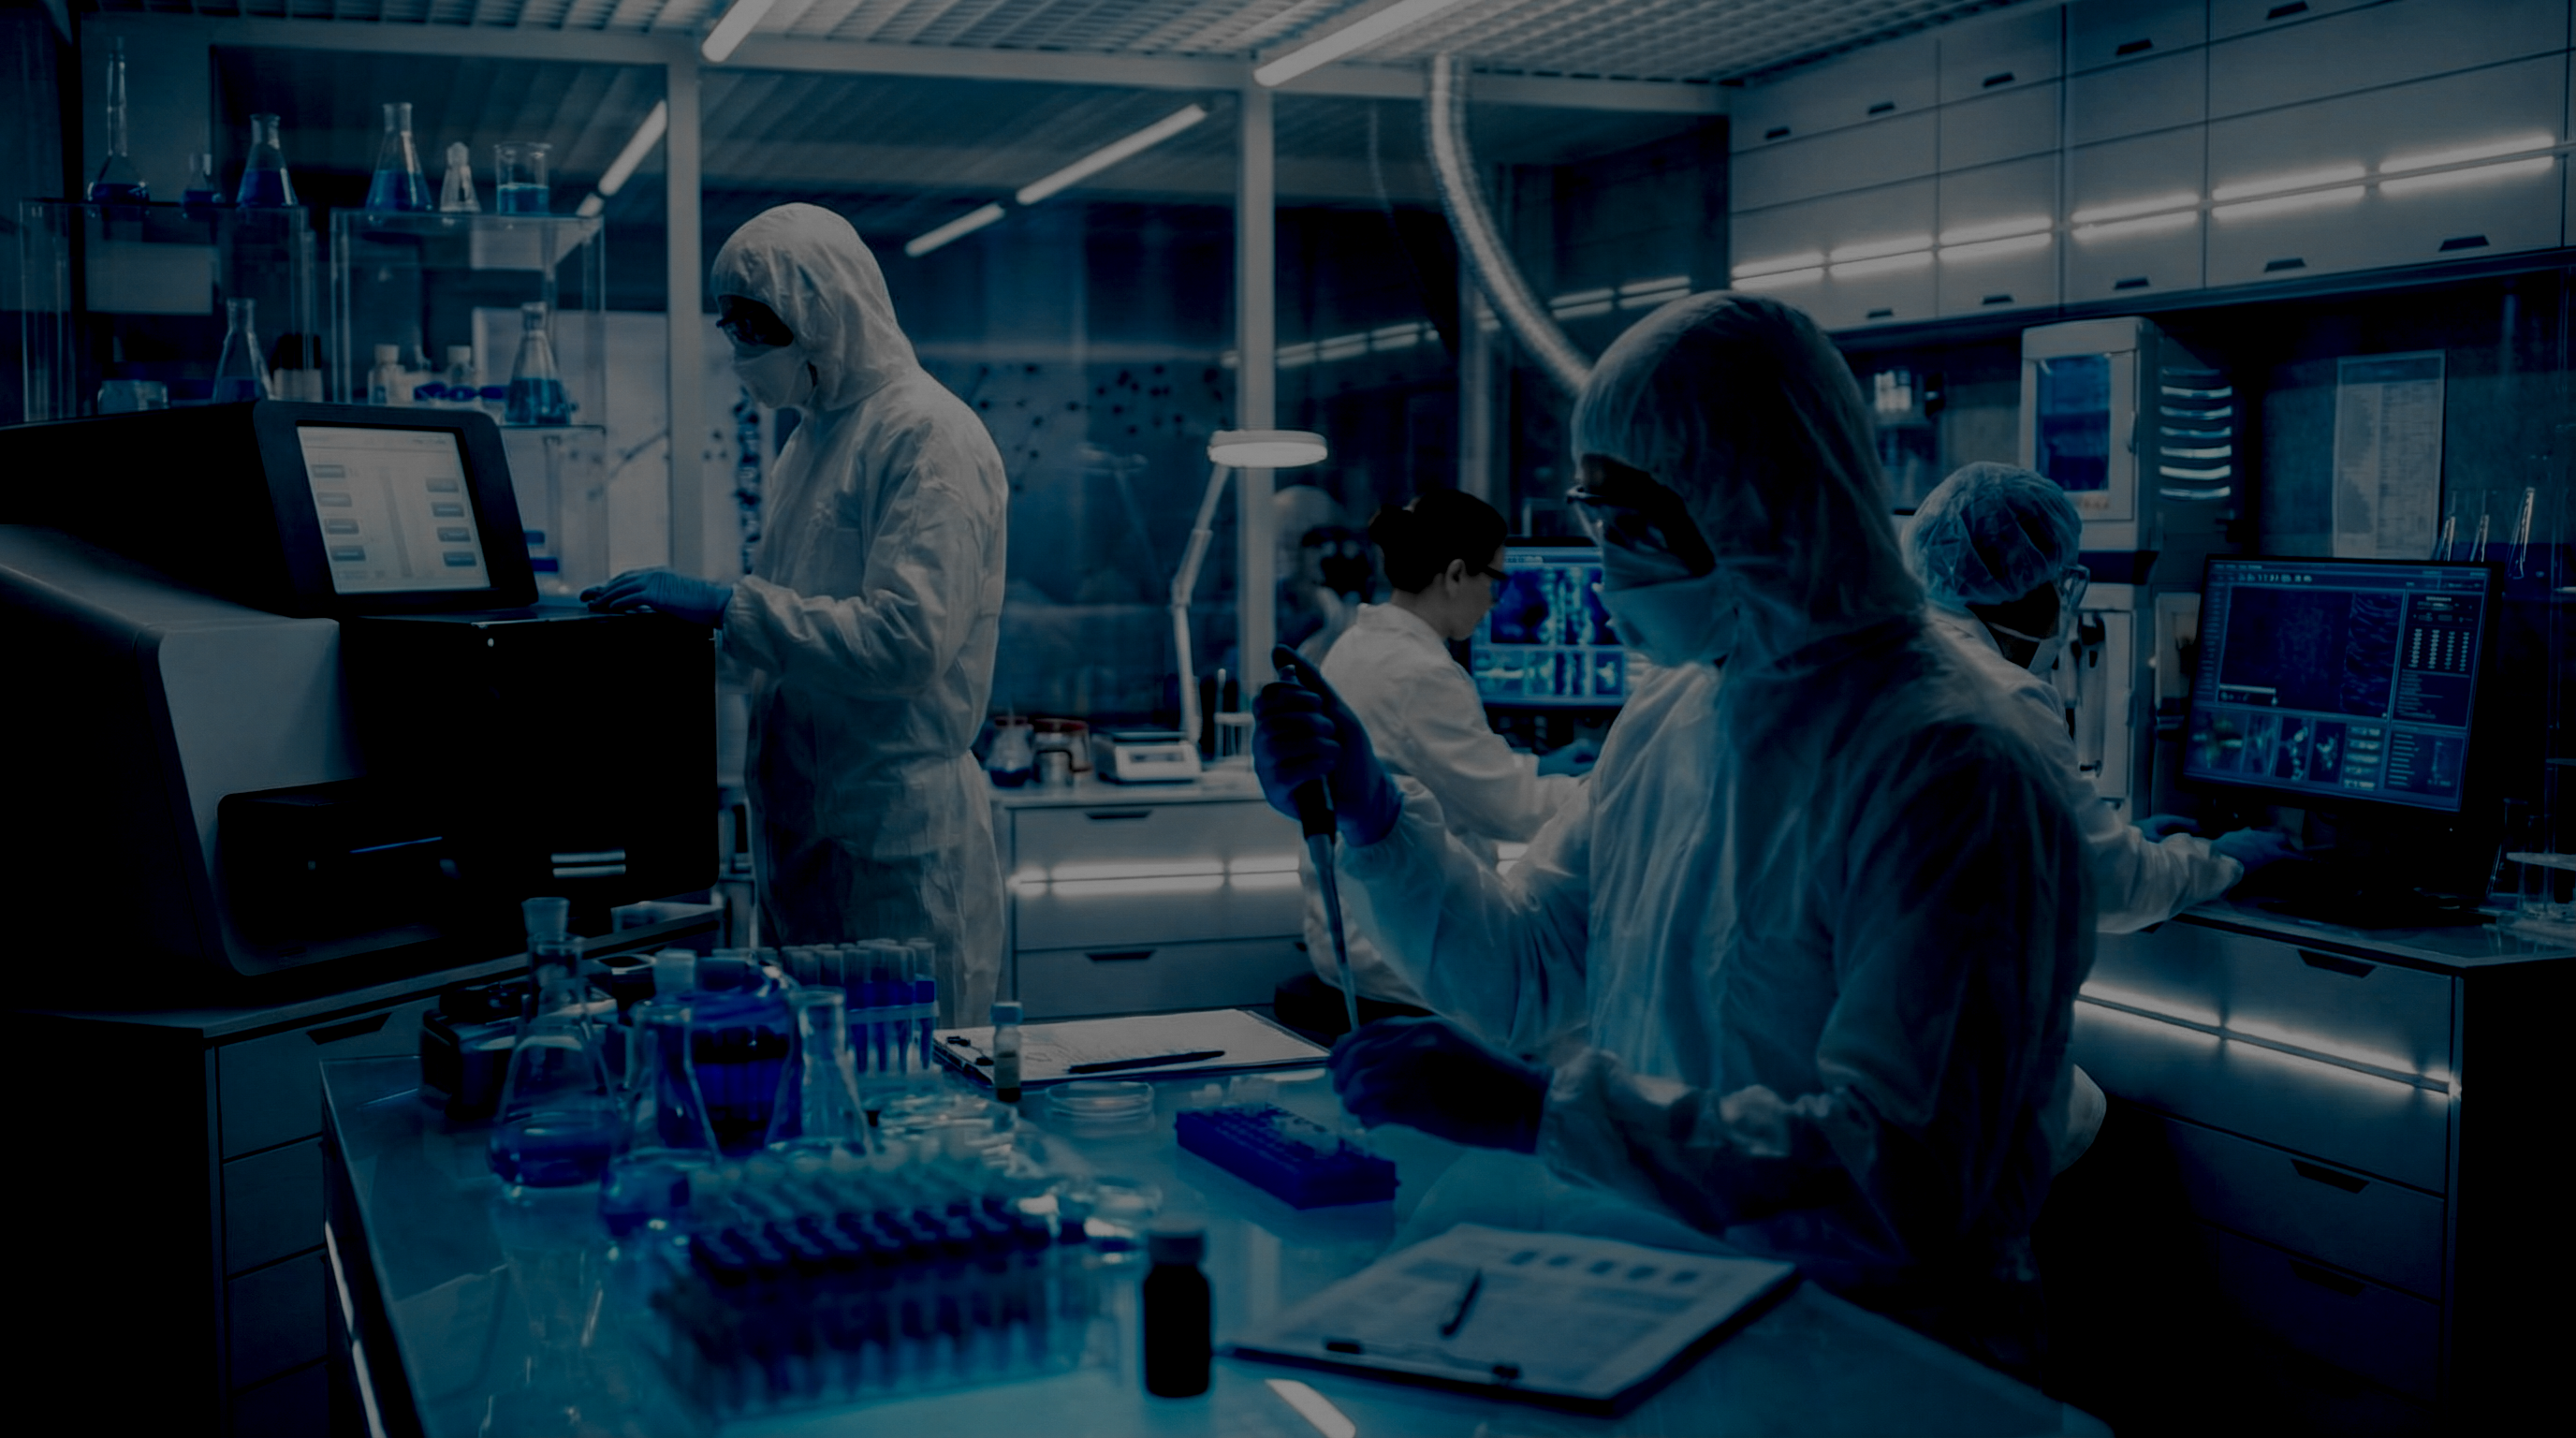
\includegraphics[width=\paperwidth,height=\paperheight]{labbackground.png}
}
\setbeamercolor{normal text}{fg=white}
\setbeamercolor{frametitle}{fg=white}
\setbeamercolor{section in toc}{fg=white}
\setbeamercolor{subsection in toc}{fg=white}
\usebeamercolor[fg]{normal text}
\begin{frame}[fragile]
\frametitle{Outline}
\tableofcontents
\end{frame}
}


\section{What is genomic data?}
\begin{frame}[plain,c]
\begin{center}
\Huge What is genomic data?
\end{center}
\end{frame}


{
\definecolor{seq_bg_gray}{rgb}{0.94, 0.94, 0.94}
\setbeamercolor{background canvas}{bg=seq_bg_gray}
\begin{frame}[fragile]
  \frametitle{What is DNA sequencing?}
  \nocite{what_is_dna_sequencing_ncbi}
  \vspace*{0cm}
  \makebox[\linewidth]{
    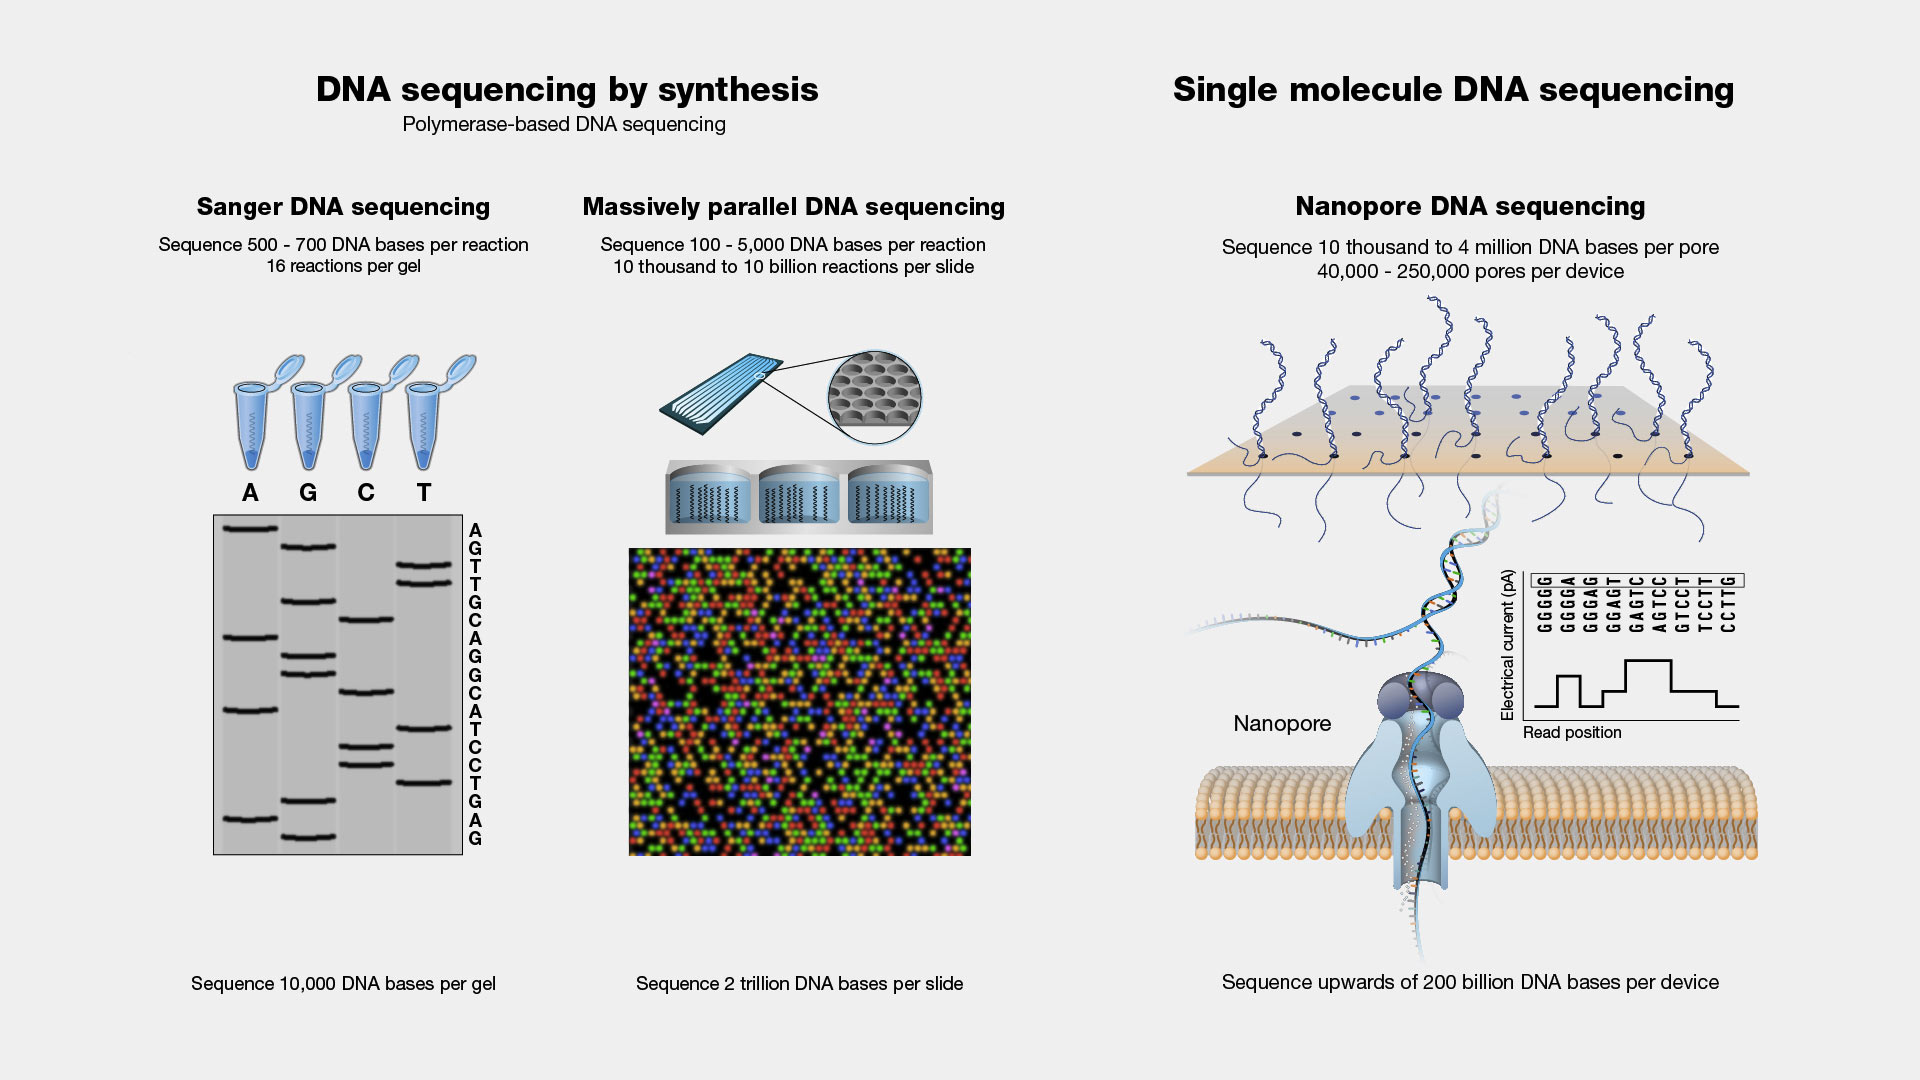
\includegraphics[scale=0.2]{whatisequencing.jpg}
  }
\end{frame}
}

\begin{frame}[fragile]
  \frametitle{Exponential growth of sequencing industry}
  \nocite{sra_getting_started}
  \nocite{ncbi_sequencing_cost_spreadsheet}

  \begin{figure}[ht]
    \centering
    \begin{CacheMeCode}{python, custom include command={\input{\robExtAddCachePathAndName{\robExtFinalHash.pgf}}}, set placeholder eval={__LINEWIDTH__}{\lenToCmNoUnit[in]{\linewidth}}}
      import matplotlib.pyplot as plt
      import matplotlib
      import numpy as np
      import json
      import pandas as pd
      from datetime import timedelta
      matplotlib.use("pgf")
      matplotlib.rcParams.update({
        "font.family": "serif",
        "font.serif": [],
        "text.usetex": True,
      })
      sra_data = pd.read_csv('../sra_stat.csv')
      costs_data = pd.read_csv('../genome_seq_costs.csv')
      fig, ax = plt.subplots()
      fig.set_size_inches(__LINEWIDTH__, 0.7*__LINEWIDTH__, forward=True)

      costs_data['date'] = pd.to_datetime(costs_data['date'], format='%b-%y')
      costs_data = costs_data[(costs_data['date'].dt.year >= 2002)]
      costs_data.set_index(['date'],inplace=True)

      sra_data['date'] = pd.to_datetime(sra_data['date'], format='%m/%d/%Y')
      #sra_data.set_index(['time'],inplace=True)\
      sra_data['year'] = pd.DatetimeIndex(sra_data['date']).year
      sra_data.set_index(['date'],inplace=True)
      sra_data_y = sra_data.drop_duplicates('year', keep='first')

      ax.plot(sra_data.index, sra_data.bases, label='All')
      ax.plot(sra_data.index, sra_data.open_access_bases, label='Open access')

      last_used_val = -100000
      rows = list(enumerate(sra_data_y.iterrows()))
      for (index, (date, row)) in rows:
          annotation_delta = timedelta(days=365)
          if index > len(rows) - 3:
              annotation_delta = timedelta(days=-365)
          xy = (date + annotation_delta, row['bases'] * 0.7)
          size_val = row['bytes'] / (1024**3)
          if (size_val - last_used_val) > size_val * 0.9:
              last_used_val = size_val
          else:
              continue
          size_unit = "GB"
          if size_val > 1024:
              size_val = size_val/1024
              size_unit = "TB"
          if size_val > 1024:
              size_val = size_val/1024
              size_unit = "PB"
          size_val = int(size_val) / 1
          #ax.annotate(f"{size_val} {size_unit}", xy=xy, textcoords='data')
          t = ax.text(
              xy[0], xy[1],
              f"{size_val} {size_unit}", 
              color='black', 
              bbox=dict(facecolor='white', edgecolor='black', boxstyle='round,pad=0.22'),
              fontsize=6,
          )
      ax.set_yscale('log')

      # US dollar cost per base
      total_cost_data_y = []
      total_cost_data_x = []
      cost_list_date = costs_data.index.to_list()
      cost_list_val_mb = costs_data['cost_per_mb_usd'].to_list()
      for (index, (date, row)) in list(enumerate(sra_data.iterrows())):
          cur_cost = cost_list_val_mb[0]
          for (l_index, lookup_date) in enumerate(cost_list_date):
              if date >= lookup_date:
                  cur_cost = cost_list_val_mb[l_index]
          #total_build_cost = cur_cost # row['bases'] / 1000000 * cur_cost
          total_build_cost = row['bases'] / 1000000 * cur_cost    
          total_cost_data_x.append(date)
          total_cost_data_y.append(total_build_cost)

      ax2 = ax.twinx()  # instantiate a second axes that shares the same x-axis
      color = 'tab:red'
      ax2.set_ylabel('USD value of all sotred data (based on avg. seq. costs)', color=color, fontsize=8)  # we already handled the x-label with ax1
      #ax2.plot(total_cost_data_x, total_cost_data_y, color=color)
      ax2.plot(total_cost_data_x, total_cost_data_y, color=color)
      ax2.tick_params(axis='y', labelcolor=color)
      ax2.set_yscale('log')
      #fig.tight_layout()  # otherwise the right y-label is slightly clipped

      # Add indicator of wehn SRA became public
      ax2.text(
        #total_cost_data_x[0],
        pd.Timestamp('04/05/2006'),
        total_cost_data_y[0]*0.1, "SRA Available to the public", rotation=90, verticalalignment='center',
        fontsize=8,
      )
      ax2.vlines(x=pd.Timestamp('06/05/2007'), ymin=0, ymax=total_cost_data_y[0]*2, color = '0')
      # End


      ax2.set_zorder(10)
      ax.set_zorder(11)
      ax.patch.set_visible(False)

      ax.set_ylabel('Number of bases', fontsize=8)
      ax.set_title("Size of NCBI SRA (Sequence Read Archive)", fontsize=8)
      ax.legend(title='Type', fontsize=8)

      print(get_filename_from_extension(".pgf"))
      plt.savefig(get_filename_from_extension(".pgf"), bbox_inches="tight")
    \end{CacheMeCode}
  \end{figure}
\end{frame}

\section{What is sequence alignment?}
\begin{frame}[plain,c]
\begin{center}
\Huge What is sequence alignment?
\end{center}
\end{frame}

{
\begin{frame}[fragile]
  \frametitle{How sequences look like?}
  \begin{texshade}{example.msf}
    \setends{1}{414..443}
    \threshold[80]{50}
    \showsequencelogo{top}
    \shadingmode[DNA]{functional}
    \showruler{top}{1} \rulersteps{1}
    \hidenumbering
    \showconsensus[ColdHot]{bottom}
    \defconsensus{.}{lower}{upper}
    \showlegend
  \end{texshade}
\end{frame}
}

% TODO: READ
% https://academic.oup.com/bioinformatics/article/41/3/btaf112/8075120
% https://www.sciencedirect.com/science/article/pii/S157086671300083X
% motif?  https://www.sciencedirect.com/science/article/pii/S1319157820305553 and here: https://pubmed.ncbi.nlm.nih.gov/24479443/ 
\begin{frame}[fragile]
  \frametitle{Alignment throughput problem}
  \begin{itemize}
    \item We can perform alignment in general case using dynamic programming in $O(nm/2)$ \footcite{ncbi_lecture_pairwise_alignment} time and space 
    \item If the distance is bounded by $k$ (Landau and Vishkin) we can do $O(nk)$
    \item If nucleotides are never added/removed we can find a match in $O(n \sqrt{k \log k})$ (Nicole Rajasekaran (2015) TODO)
  \end{itemize}
\end{frame}


\section{Problem statement and master thesis plan}

\begin{frame}{Solutions comparison}
  \begin{table}[!htb]
    % \setlist[itemize]{nosep,
    %   leftmargin=*,
    %   label=\textbullet,
    %   after =\vspace{-\baselineskip},% <---
    %   before=\vspace{-\baselineskip} % <---
    % }
    \fontsize{6}{2}\selectfont
    \begin{tblr}{
      hlines, vlines,
      colspec = {Q[l,m] X[l,h] X[l,h]},
      row{1} = {font=\bfseries},
      measure = vbox
    }
    Methods & Pro & Cons \\
    % BLAST+
    %     & \begin{itemize}
    %       \item Actively maintained
    %       \item Popular software
    %     \end{itemize}
    %     & \begin{itemize}
    %       \item Written in 19XX 
    %       \item Does not use latest SoTA optimisations
    %     \end{itemize} \\
    MonetDB/MariaDB/MySQL
        & \begin{itemizesmall}
          \item Popular databases
        \end{itemizesmall}
        & \begin{itemizesmall}
          \item Need to specify schema 
          \item Cannot directly store long sequences 
          \item Need custom storage interface to load/store data
        \end{itemizesmall}\vspace{\baselineskip} \\
    S3 with FASTA files
        & \begin{itemizesmall}
          \item Most common format directly accessible by most of the tools
          \item Used by BLAST+ and most other NCBI search tools
        \end{itemizesmall}
        & \begin{itemizesmall}
          \item Local unversioned files cause problem with experiments' reproducibility
          \item Sometimes very big and stored in uncompressed plaintext
          \item Slow to process
          \item No standard metadata format
        \end{itemizesmall}\vspace{\baselineskip} \\
    Dedicated DBMS
        & \begin{itemizesmall}
          \item ?
        \end{itemizesmall}
        & \begin{itemizesmall}
          \item Mostly using combination of both methods
          \item Not popular
        \end{itemizesmall}\vspace{\baselineskip} \\
    \end{tblr}
  \end{table}
\end{frame}

\begin{frame}[fragile]
\definecolor{myblue}{rgb}{0.2,0.2,0.7}
\definecolor{myred}{rgb}{0.2,0.2,0.7}
\definecolor{mygreen}{rgb}{0.2,0.2,0.7}
\definecolor{myviolet}{rgb}{0.2,0.2,0.7}
\definecolor{myturquoise}{rgb}{0.2,0.2,0.7}
\definecolor{myorange}{rgb}{0.2,0.2,0.7}
\begin{tikzpicture}[myarrow/.style={single arrow,single arrow head extend=.1cm,anchor=west,minimum height=.8cm,minimum width=.8cm},
    mycircle/.style={circle,text=white,inner sep=.2cm,outer sep=.2cm,minimum width=2.5cm}]
\begin{scope}[shift = {(9, 0)}]
\node(a)[draw=myblue,mycircle,fill=myblue,circle,text=white,inner sep=.2cm,outer sep=.2cm]{BioSeqDB};
\node(b)[draw=myturquoise,fill=myturquoise,myarrow,rotate=220]at(a.220){};
\node(c)[draw=myviolet,fill=myviolet,myarrow,rotate=320]at(a.320){};
\node(d)[draw=mygreen,fill=mygreen,myarrow,rotate=30]at(a.30){};
\node(e)[draw=myorange,fill=myorange,myarrow,rotate=150]at(a.150){};
\node(f)[draw=myred,fill=myred,myarrow,rotate=90]at(a.90){};
\node(g)[text width=6em,text centered,font=\small,draw=myred,fill=myred,mycircle,anchor=south]at(f.east){Postgres \\ advantages \\ for metadata};
\node(g)[text width=6em,text centered,font=\small,draw=myorange,fill=myorange,mycircle,anchor=-40]at(e.east){Faster \\ alignment \\ of sequences};
\node(g)[text width=6em,text centered,font=\small,draw=myviolet,fill=myviolet,mycircle,anchor=140]at(c.east){Incremental \\ index \\ building};
\node(g)[text width=6em,text centered,font=\small,draw=mygreen,fill=mygreen,mycircle,anchor=-140]at(d.east){Easy \\ setup};
\node(g)[text width=6em,text centered,font=\small,draw=myturquoise,fill=myturquoise,mycircle,anchor=40]at(b.east){Querying \\ via SQL};
\end{scope}
\end{tikzpicture}
\end{frame}


% \begin{frame}
% \frametitle{\centerline{Problem statement}}

% \smartdiagramset{planet font=\sffamily\Huge,
%    satellite font=\sffamily,
%    planet color=green!40, uniform connection color=true,
%    uniform color list = red!40 for 8 items}
% \tikzset{satellite/.append style={regular polygon,
%   regular polygon sides=8, inner sep=0pt},
%   planet/.append style={regular polygon,
%   regular polygon sides=8, inner sep=6pt}}
% \smartdiagram[constellation diagram]{BioSeqDB,
%   Metadata in relations, Sequences storage, Familiar SQL processing, Optimized for large sequences }

% \end{frame}

\begin{frame}
\frametitle{\centerline{Master thesis timeline}}
\begin{table}
\renewcommand\arraystretch{1.4}\arrayrulecolor{black}
\begin{tabular}{c @{\,}r <{\hskip 2pt} !{\foo} >{\raggedright\arraybackslash}p{5cm}}
\toprule
\addlinespace[1.5ex]
$\checkmark$ & May 2024 & Stage I: Writing my own aligner in Python \\
$\checkmark$ & Nov 2025 & Stage II: Integrating Postgres  \\
$\,\to\,$ & Dec 2025 & Stage III: Custom storage  \\
& Feb 2025 & Stage IV: Heuristic-based algorithm selection \\
& Apr 2025 & Stage V: Benchmarking and GTM \\
& May 2025 & Finalization \\
\end{tabular}
\end{table}
\end{frame}

\section{Modern aligners}

\begin{frame}[fragile]
  \frametitle{Seed and Extend approach}
  \nocite{blend}

  \begin{center}
    \begin{tikzpicture}[scale=.6, transform shape, node distance=1cm, >=Latex, overlay, remember picture, shift={(0,3.5)}]

      \node (ap1title) at (0,2) {(k,w)-minimizers};
      \draw[rounded corners=3pt]
      (ap1title) -| (-8.5,-2) -| (8.5,2) -- (ap1title);
  
      \node (ap2title) at (0,-2.5) {Spacing};
      \draw[rounded corners=3pt]
      (ap2title) -| (-8.5,-6.5) -| (8.5,-2.5) -- (ap2title);
  
      \node (ap3title) at (0,-7) {Strobomers};
      \draw[rounded corners=3pt]
      (ap3title) -| (-8.5,-11) -| (8.5,-7) -- (ap3title);
    
      \node(k1)[tinybox, colprimaryl, below left=0.4cm and 3cm of ap1title]{GCTATTA};
      \node(k2)[tinybox, colprimaryl, below right=0.1cm and -1.7cm of k1]{CTATTAC};
      \node(k3)[tinybox, colprimaryl, below right=0.1cm and -1.7cm of k2]{TATTACC};
      \node(k4)[tinybox, colprimaryl, below right=0.1cm and -1.7cm of k3]{ATTACCT};
  
      \node(h1)[tinybox, colprimary, right=1.5cm of k1]{Hash};
      \node(h2)[tinybox, colprimary, below=0.1cm of h1]{Hash};
      \node(h3)[tinybox, colprimary, below=0.1cm of h2]{Hash};
      \node(h4)[tinybox, colprimary, below=0.1cm of h3]{Hash};
  
      \node(h1v)[tinybox, right=1.5cm of h1]{\texttt{0xA1}};
      \node(h2v)[tinybox, below=0.1cm of h1v]{\texttt{0x02}};
      \node(h3v)[tinybox, below=0.1cm of h2v]{\texttt{0xFC}};
      \node(h4v)[tinybox, below=0.1cm of h3v]{\texttt{0x45}};
  
      \draw[->](k1)--(h1);
      \draw[->](k2)--(h2);
      \draw[->](k3)--(h3);
      \draw[->](k4)--(h4);
  
      \draw[->](h1)--(h1v);
      \draw[->](h2)--(h2v);
      \draw[->](h3)--(h3v);
      \draw[->](h4)--(h4v);
  
      \node(min)[operation, minimum width=1cm, minimum height=2.5cm, below right=-0.5cm and 1.5cm of h1v]{Find Min};
  
      \draw[fork](h1v.east)--(min.west);
      \draw[fork](h2v.east)--(min.west);
      \draw[fork](h3v.east)--(min.west);
      \draw[fork](h4v.east)--(min.west);
  
      \node(minh)[tinybox, right=4.5cm of h1v]{\texttt{0x02}};
      \draw[->](min.east) |- ++(0.3cm, 0mm) coordinate(min) |- (minh.west);
  
      \node(minmer)[tinybox, colprimaryl, below=1.3cm of minh]{CTATTAC};
      \draw[->](minh)--(minmer);
  
      % BOX
      \node (seedbox1)[below=0.1cm of minmer] {Seed: Minimizer};
      \draw[rounded corners=3pt] (seedbox1) -| ++(-1.5cm, 1.3cm) coordinate(seedbox1) -| ++(2.9cm, -1.3cm) coordinate(seedbox1) |- ++(-0.2cm, 0cm) coordinate(seedbox1);
  
      % Second one
  
      \node(spk1)[tinybox, colprimaryl, below left=0.4cm and 3cm of ap2title]{GCTATTA};
      \node(spk2)[tinybox, colprimaryl, below=0.1cm of spk1]{GATACTA};
      \node(spk3)[tinybox, colprimaryl, below=0.1cm of spk2]{GACACTA};
  
      \node(p1)[tinybox, right=0.9cm of spk1]{Pattern};
      \node(p2)[tinybox, below=0.1cm of p1]{Pattern};
      \node(p3)[tinybox, below=0.1cm of p2]{Pattern};
  
      \node(sps1)[tinybox, colprimaryl, right=0.9cm of p1]{G\hl{\textbf{X}}TA\hl{\textbf{X}}TA};
      \node(sps2)[tinybox, colprimaryl, below=0.1cm of sps1]{G\hl{\textbf{X}}TA\hl{\textbf{X}}TA};
      \node(sps3)[tinybox, colprimaryl, below=0.1cm of sps2]{G\hl{\textbf{X}}CA\hl{\textbf{X}}TA};
  
      % BOX
      \node (seedbox2)[below=0.9cm of sps2] {Seeds: Spaced};
      \draw[rounded corners=3pt] (seedbox2) -| ++(-1.5cm, 2.8cm) coordinate(seedbox2) -| ++(2.9cm, -2.8cm) coordinate(seedbox2) |- ++(-0.2cm, 0cm) coordinate(seedbox2);
  
      \node(sh1)[tinybox, colprimary, right=0.9cm of sps1]{Hash};
      \node(sh2)[tinybox, colprimary, below=0.1cm of sh1]{Hash};
      \node(sh3)[tinybox, colprimary, below=0.1cm of sh2]{Hash};
  
      \node(sh1v)[tinybox, right=0.9cm of sh1]{\texttt{0xA1}};
      \node(sh2v)[tinybox, below=0.1cm of sh1v]{\texttt{0xA1}};
      \node(sh3v)[tinybox, below=0.1cm of sh2v]{\texttt{0xFC}};
  
      \draw[->](spk1)--(p1);
      \draw[->](spk2)--(p2);
      \draw[->](spk3)--(p3);
  
      \draw[->](p1)--(sps1);
      \draw[->](p2)--(sps2);
      \draw[->](p3)--(sps3);
  
      \draw[->](sps1)--(sh1);
      \draw[->](sps2)--(sh2);
      \draw[->](sps3)--(sh3);
  
      \draw[->](sh1)--(sh1v);
      \draw[->](sh2)--(sh2v);
      \draw[->](sh3)--(sh3v);
  
      % Third 
  
      \node(stk1)[tinybox, colprimaryl, below left=0.4cm and 0.7cm of ap3title]{\hl{\textbf{GCTA}}TTACC\hl{\textbf{TTAA}}TGTGA\hl{\textbf{TGGA}}C};
      \node(stk2)[tinybox, colprimaryl, below=0.1cm of stk1]{\hl{\textbf{GCTA}}TCCCC\hl{\textbf{TTAA}}TGGGA\hl{\textbf{TGGA}}C};
      \node(stk3)[tinybox, colprimaryl, below=0.1cm of stk2]{GC\tikzmark{stk3h1b}\hl{\textbf{CCTC}}\tikzmark{stk3h1e}CCCT\tikzmark{stk3h2b}\hl{\textbf{TAAA}}\tikzmark{stk3h2e}GGGA\tikzmark{stk3h3b}\hl{\textbf{TGGA}}\tikzmark{stk3h3e}C};
  
      \node(stkdescription)[below=0.4cm of stk3]{Selected k-mers};
  
      \path let \p1=($(pic cs:stk3h1b)!0.5!(pic cs:stk3h1e)$), \p2=($(stkdescription)!0.5!(stk3)$) in ($ (\x1, \y2) - (7, 0) $) |- (stkdescription) coordinate [pos=0] (stk3h1x);
      \path let \p1=($(pic cs:stk3h2b)!0.5!(pic cs:stk3h2e)$), \p2=($(stkdescription)!0.5!(stk3)$) in ($ (\x1, \y2) - (5, 0) $) |- (stkdescription.north) coordinate [pos=0] (stk3h2x);
      \path let \p1=($(pic cs:stk3h3b)!0.5!(pic cs:stk3h3e)$), \p2=($(stkdescription)!0.5!(stk3)$) in ($ (\x1, \y2) - (3, 0) $) |- (stkdescription) coordinate [pos=0] (stk3h3x);
      \draw (stk3h1x) |- (stkdescription.west);
      \draw (stk3h2x) |- (stkdescription.north);
      \draw (stk3h3x) |- (stkdescription.east);
  
      \node(l1)[tinybox, right=0.6cm of stk1]{Link};
      \node(l2)[tinybox, below=0.1cm of l1]{Link};
      \node(l3)[tinybox, below=0.1cm of l2]{Link};
  
      \node(sts1)[tinybox, colprimaryl, right=0.6cm of l1]{GCTATTAATGGA};
      \node(sts2)[tinybox, colprimaryl, below=0.1cm of sts1]{GCTATTAATGGA};
      \node(sts3)[tinybox, colprimaryl, below=0.1cm of sts2]{CCTCTAAATGGA};
  
      % BOX
      \node (seedbox3)[below=1cm of sts2] {Seeds: Strobomers};
      \draw[rounded corners=3pt] (seedbox3) -| ++(-2cm, 2.8cm) coordinate(seedbox3) -| ++(3.8cm, -2.8cm) coordinate(seedbox3) |- ++(-0.2cm, 0cm) coordinate(seedbox3);
  
      \node(sth1)[tinybox, colprimary, right=0.6cm of sts1]{Hash};
      \node(sth2)[tinybox, colprimary, below=0.1cm of sth1]{Hash};
      \node(sth3)[tinybox, colprimary, below=0.1cm of sth2]{Hash};
      
      \node(sth1v)[tinybox, right=0.6cm of sth1]{\texttt{0xA1}};
      \node(sth2v)[tinybox, below=0.1cm of sth1v]{\texttt{0xA1}};
      \node(sth3v)[tinybox, below=0.1cm of sth2v]{\texttt{0xFC}};
  
      \draw[->](stk1)--(l1);
      \draw[->](stk2)--(l2);
      \draw[->](stk3)--(l3);
  
      \draw[->](l1)--(sts1);
      \draw[->](l2)--(sts2);
      \draw[->](l3)--(sts3);
  
      \draw[->](sts1)--(sth1);
      \draw[->](sts2)--(sth2);
      \draw[->](sts3)--(sth3);
  
      \draw[->](sth1)--(sth1v);
      \draw[->](sth2)--(sth2v);
      \draw[->](sth3)--(sth3v);
      
    \end{tikzpicture}
  \end{center}

\end{frame}


\section{Stage I: Writing my own aligner in Python}
\begin{frame}[plain,c]
\begin{center}
\Huge Stage I: Writing my own aligner in Python
\end{center}
\end{frame}

\begin{frame}
  \frametitle{Problem specification}

  \begin{tcolorbox}[colback=green!5,colframe=green!40!black,title=Time]
  Aligning short sequences up to 1k bases with $5\% \pm 5\%$ error rate.
  Given the reference sequence of length≤20 Mbp, a collection of reads should be processed in at most 2+r/10 minutes (max 1000 reads) (i.e avg. 6s per read) and memory<1GB
  \end{tcolorbox}
\end{frame}


\begin{frame}[fragile]
  \frametitle{Seed and Extend approach}

  {\centering
  \begin{tikzpicture}[scale=.7, transform shape, node distance=1cm, >=Latex]
    \node(LT)[bigbox]{Load target};
    \node(TI)[bigbox, right=2cm of LT]{Build target index};
    \node(LQ)[bigbox, right=2cm of TI]{Build query index};
    \node(S)[bigbox, below=of LQ]{Find seeds};
    \node(E)[bigbox, left=of S]{Extend};


    \node(X)[left=3cm of E]{};
    \node(ABWT)[smallbox, above=2.5mm of X]{BWT};
    \node(ADP)[smallbox, below=2.5mm of X]{Raw DP};

    \node(QC)[bigbox, left=3cm of X]{Quality control};
    \node(R)[bigbox, below=2cm of QC]{Report alignment};

    \draw[->](LT)--(TI);
    \draw[->](TI)--(LQ);
    \draw[->](LQ)--(S);
    \draw[->](S)--(E);
    \draw[->](QC)--(R);

    \draw[fork](E.west)--(ABWT.east);
    \draw[fork](E.west)--(ADP.east);

    \draw[fork](ABWT.west)--(QC.east);
    \draw[fork](ADP.west)--(QC.east);

    %\draw[fork](QC.south)--(ADP.south);

    \path ($(R)!0.45!(ADP)$) -| (QC) coordinate [pos=0.2] (aux);
    \draw (QC) |- (aux);
    \draw[->] (aux) -| (ADP);

  \end{tikzpicture}
  \par}
\end{frame}

\begin{frame}
  \frametitle{Aligner algorithm description}
  \scriptsize
  \begin{enumerate}
    \item Build reference index structures
    \begin{enumerate}
      \scriptsize
      \item Read reference in chunks of size $800000$
      \item For each chunk generate (k=$17$, w=$8$)-minimizer index chunk
      \item Filter out every other $15$-th k-mer (only if it occurs only once within the chunk)
      \item Merge chunk index into full reference index and repeat for other chunks
    \end{enumerate}
    \item Load query and build (k=$17$, w=$8$)-minimizer index
    \item Find common matches and generate cross-product
    \item Perform seed extension (described in detail later) and generate matching positions with scores
    \item Filter $5$ top scores $\geq 0.1$
    \begin{enumerate}
        \scriptsize
        \item For $|scores| = 0$ try building full LIS and use sliding window with highest scoring: $min(|match_q|, |match_t|)^2 - \sum {diff(match_t)}$
        \item For $|scores| = 1$ proceed normally
        \item For $|scores| > 1$ get region with lowest score generated by DP aligner
    \end{enumerate}
    \item Perform final one region matching
  \end{enumerate}

\end{frame}


\begin{frame}
  \frametitle{Aligner algorithm description}
  \scriptsize
  \begin{enumerate}
    \setcounter{enumi}{5}
    \item Perform final one region matching
    \begin{enumerate}
      \scriptsize
      \item For every region virtually resize it by $kmer\_len*0.5+1 = 9$ each side
      \item For every region do quick BWT backtrack aligment on $10\%$ of match (start and end) with max err. rate $10\%=10$
      \item If BWT finds match on end but padding exceeds $4\%$ of match length, execute DP aligner (but only on first parameter configuration i.e $(15, 11)$)
      \begin{enumerate}
        \scriptsize
        \item DP aligner takes prefix/suffix of $40\%$ of query size
        \item For $(kmer_len, step) = ((15, 11), (8, 5))$ it tries to match the pair target/sequence
        \item Run recursive algorithm with threshold of errors $\leq (|query| * 11.11\%)$
      \end{enumerate}
      \item Now if padding returned by BWT or/and DP aligners make region exceed size of $|query|*105\%$ then repeat BWT matching process with new estimate $start = found\_end - |query|$
      \item If we repeated procedure of running BWT/DP twice and came here again, then we assume there is no good match
    \end{enumerate}
    \item Filter out matches if region exceed size of $|query|*105\%$
    \item Print matches coorindates
  \end{enumerate}

\end{frame}

\begin{frame}[fragile]
  \frametitle{Minimizer generation i.e numpy magic}

  \begin{minted}[fontsize=\scriptsize]{python}
  def get_minimizers(seq_arr: NDArray[Shape["*"], UInt8]): 
      sequence_len = len(seq_arr)
      mask = generate_mask(KMER_LEN)  # Bitwise mask

      # Function to compute kmer value based on the previous
      # (on the left side) kmer value and new nucleotide
      uadd = frompyfunc(lambda x, y: ((x << 2) | y) & mask, 2, 1)
      kmers = uadd.accumulate(seq_arr, dtype=object).astype(int)
      kmers[:KMER_LEN-2] = 0
      
      # Do sliding window and get min kmers positions
      kmers_min_pos = add(
          argmin(
            sliding_window_view(kmers, window_shape=WINDOW_LEN
          ), axis=1),
          arange(0, sequence_len - WINDOW_LEN + 1)
      )
      
      # ...
  \end{minted}
\end{frame}

\begin{frame}[fragile]
  \frametitle{Minimizer generation i.e numpy magic}

  \begin{minted}[fontsize=\tiny]{python}
      # ...
      # Now collect all selected mimumum and kmers into single table
      selected_kmers = column_stack((
        kmers[kmers_min_pos],
        kmers_min_pos,
      ))[KMER_LEN:].astype(uint32)

      # Remove duplicates
      selected_kmers = selected_kmers[selected_kmers[:, 0].argsort()]
      selected_kmers = unique(selected_kmers, axis=0)

      # This part performs "group by" using the kmer value
      selected_kmers_unique_idx = unique(
        selected_kmers[:, 0], return_index=True
      )[1][1:]
      selected_kmers_entries_split = split(selected_kmers[:, 1], selected_kmers_unique_idx)

      if len(selected_kmers) == 0:
          return dict()
      return dict(zip(
        chain([selected_kmers[0, 0]], selected_kmers[selected_kmers_unique_idx, 0]),
        selected_kmers_entries_split
      ))
  \end{minted}
\end{frame}



\begin{frame}[fragile]
  \frametitle{Bonus: we can encode sequence signature as List[uint64]}
  \fboxsep=0pt
  \noindent
  \begin{minipage}[t]{0.48\linewidth}
    \vspace{0.8cm}
    \begin{enumerate}
      \scriptsize
      \item (1 bit) Flag for min/max
      \item (45 bits) Kmer hash value
      \item (16 bits) Number of occurences
      \item (1 bit) Flags for margin test/train
    \end{enumerate}

  \end{minipage}
  \hfill
  \begin{minipage}[t]{0.48\linewidth}
    \begin{algorithm}[H]
      \captionsetup{font=scriptsize}
      \caption{Test}
      \scriptsize
      \begin{algorithmic}
        \State $x \gets kmer\_{hash} \BitAnd mask_{kmer}$
        \State $x \gets x \ShiftLeft 16$
        \State $x \gets x \BitOr (kmer\_{count} \BitAnd mask_{count})$
        \State $x \gets x \ShiftLeft 1$
        \State $x \gets x \BitOr kmer_{is\_test}$
        \State $x \gets x \BitOr (kmer_{is\_max} \ShiftLeft 62)$
      \end{algorithmic}
    \end{algorithm}
  \end{minipage}

  \begin{center}
    \vspace{0.4cm}
    \begin{bytefield}[bitwidth=0.027\linewidth]{38}
      \bithead{1}{1} & \bithead{20}{45} &
      \bithead{7}{16} & \bithead{1}{1}\\
      \bitbox{1}{} & \bitbox{20}{20-mer} &
      \bitbox{7}{Occ Count} & \bitbox{1}{}\\
      \bitbox[]{1}{$\smallunderbrace{\hspace{0.027\linewidth}}_{\mathrlap{\text{\normalsize Train/Test}}}$} & \bitbox[]{20}{} &
      \bitbox[]{7}{} & \bitbox[]{1}{$\smallunderbrace{\hspace{0.027\linewidth}}_{\mathllap{\text{\normalsize Min/Max}}}$}\\
    \end{bytefield}
  \end{center}
\end{frame}

\begin{frame}[fragile]
  \frametitle{Bonus: we can encode sequence signature as List[uint64]}
  \begin{tcolorbox}[fontlower=\tiny, colback=green!5,colframe=green!40!black,title=Bonus!]
    We then have short signature vectors representing single sequence or entire sets of sequences.
    This means we can do LSH to detect similarity of sequences' datasets (easy clsutering) and predict evolutionary direction.
  \end{tcolorbox}
\end{frame}

\begin{frame}
  \frametitle{Problem of extending seeds}

  \begin{itemize}
    \item minimap2 \footcite{minimap2} approach with dynamic programming similar to normal alignment (plus exponential forward lookups)
    \item We have only one potential match so maybe assume that $match \in LIS(matches)$
    \item Can we formulate sliding window approach to generate the biggest scorring windows included in $LIS(matches)$?
    \item For which case assumption that $match \in LIS(matches)$ won't work?
    \item Can we modify LIS to perhaps include other potential matches?
  \end{itemize}
\end{frame}

\begin{frame}
  \frametitle{Seed extension}
  
  \begin{algorithm}[H]
      \captionsetup{font=scriptsize}
      \caption{Standard LIS construction O(n log n)}\label{alg:cap}
      \scriptsize
      \begin{algorithmic}
          \Require $n \geq 0$
          %\Ensure $y = x^n$
          \State $lis\_len \gets 0$ \Comment{Length of LIS}
          \State $parent \gets \{\infty, \infty, \infty, ..., \infty\}_{n+1}$ \Comment{Mapping to reconstruct LIS}
          \State $sub \gets \{\infty, \infty, \infty, ..., \infty\}_{n+1}$ \Comment{Array with indices for matches that form LIS}
          \State $i \gets 0$
          \While{$i < n$} \Comment{Iterate over all elements $i = 0, 1, 2..., n-1$}
              \State $start \gets 1$
              \State $end \gets lis\_len$
              \While{$start \leq end$} \Comment{Binary search over existing longest sequence}
                  \State $middle \gets \floor*{\frac{start + end}{2}}$
                  \If{$matches_{q}[sub[middle]] < matches_{q}[i]$}
                      \State{$start \gets middle + 1$}
                  \Else
                      \State{$start \gets middle - 1$}
                  \EndIf
              \EndWhile
              \State{$parent[i] \gets sub[start-1]$} \Comment{We pin current value to the found parent}
              \State{$sub[start] \gets i$}
              \If{$start > lis\_len$}
                  \State{$lis\_len = start$}
              \EndIf
              \State{$i \gets i+1$}
          \EndWhile
      \end{algorithmic}
  \end{algorithm}
\end{frame}

\begin{frame}
  \frametitle{Seed extension}
  \begin{algorithm}[H]
    \caption{Reconstruct LIS by following parent array O(n)}\label{alg:cap}
    \begin{algorithmic}
        \State{$current\_node \gets sub[lis\_len]$}
        \State{$result \gets \{0, 0, 0,..., 0\}_{lis\_len}$}
        \State{$result[lis\_len-1] \gets current\_node$} \Comment{Will contain all indices from matches describing the output subsequence}
        \State{$j \gets lis\_len-1 $}
        \While{$1 \leq j$}
            \State{$current\_node \gets parent[current\_node]$}
            \State{$result[j-1] \gets current\_node$}
            \State{$j \gets j-1$}
        \EndWhile
    \end{algorithmic}
  \end{algorithm}
\end{frame}

\begin{frame}[fragile]
  \frametitle{Seed extension (unwanted case)}

  \begin{center}
    \begin{tikzpicture}[scale=.6, transform shape, node distance=1cm, >=Latex, remember picture]

      \node(kstart)[]{};
      \node(k1)[tinybox, right=0.5cm of kstart, align=center]{$k_1$\\$10-80$};
      \node(k2)[tinybox, right=0.5cm of k1, align=center]{$k_2$\\$90-142$};
      \node(k3)[tinybox, right=0.5cm of k2, align=center]{$k_3$\\$150-233$};
      \node(k4)[tinybox, colprimary, right=0.9cm of k3, align=center]{$k_4 (l=562)$\\$239-801$};
      \node(k5)[tinybox, right=0.9cm of k4, align=center]{$k_5$\\$602-605$};
      \node(k6)[tinybox, colprimary, right=0.9cm of k5, align=center]{$k_6 (l=691)$\\$306-997$};
      \node(k7)[tinybox, right=0.5cm of k6, align=center]{$k_7$\\$950-960$};
      \node(kend)[right=0.5cm of k7]{};
  
      \draw[->](kstart)--(k1);
      \draw[-](k1)--(k2);
      \draw[-](k2)--(k3);
      \draw[-](k3)--(k4);
      \draw[-](k4)--(k5);
      \draw[-](k5)--(k6);
      \draw[-](k6)--(k7);
      \draw[->](k7)--(kend);
  
      \node(desctail)[below=0.6cm of k2]{Unwanted tail};
      \draw (k1) |- (desctail.west);
      \draw (k2) -- (desctail.north);
      \draw (k3) |- (desctail.east);
  
      \node(desck4)[below=1.2cm of k4]{Worse candidate compared to $k6$};
      \draw (k4) -- (desck4.north);
  
      \node(desck6)[below=0.6cm of k6]{Will be cut to $606-997 (l=391)$ because of the tail};
      \draw (k6) -- (desck6.north);
  
      \node (listitle)[below right=3cm and 1.5cm of k1]{LIS vs what we want};
      \draw[rounded corners=3pt]
      (listitle) -| ++(-3cm, -2cm) coordinate(listitle) -| ++(15cm, 2cm) coordinate(listitle) -- ++(-10cm, 0cm) coordinate(listitle);
  
      \node(listext1)[below right=0.35cm and -4.2cm of listitle]{$LIS([k_1,...k_7]) = [ (10, 80); (90; 142); (150; 233); $\hl{(239; 801)}$; $\hl{(802, 997)}$ ]$};
  
      \node(listext2)[below=0.1cm of listext1]{$LIS'([k_1,...k_7]) = [ (10, 80); (90; 142); (150; 233); $\hl{(239; 400)}$; $\hl{(401, 997)}$ ]$};
      
    \end{tikzpicture}
  \end{center}

\end{frame}

\begin{frame}
  \frametitle{Seed extension (heuristic)}
  
  \begin{algorithm}[H]
      \captionsetup{font=scriptsize}
      \caption{Segmented-LIS heuristic O(n log n)}\label{alg:cap}
      \tiny
      \begin{algorithmic}
          \Require $n \geq 0$
          %\Ensure $y = x^n$
          \State $lis\_len \gets 0$ \Comment{Length of LIS}
          \State $parent \gets \{\infty, \infty, \infty, ..., \infty\}_{n+1}$ \Comment{Mapping to reconstruct LIS}
          \State $sub \gets \{\infty, \infty, \infty, ..., \infty\}_{n+1}$ \Comment{Array with indices for matches that form LIS}
          \State $i \gets 0$
          \While{$i < n$} \Comment{Iterate over all elements $i = 0, 1, 2..., n-1$}
              \State $start \gets 1$
              \State $end \gets lis\_len$
              \While{$start \leq end$} \Comment{Binary search-like}
                  \State $middle \gets \floor*{\frac{start + end}{2}}$
                  \If{$matches_{T}[sub[middle]] > matches_{T}[i] - max\_diff$} \Comment{Encountered old entry}
                      \State{$end \gets start - 1$} \Comment{Breaks loop}
                  \ElsIf{$matches_{Q}[sub[middle]] < matches_{Q}[i]$}
                      \State{$start \gets middle + 1$}
                  \Else
                      \State{$start \gets middle - 1$}
                  \EndIf
              \EndWhile
              \State{$parent[i] \gets sub[start-1]$} \Comment{We pin current value to the found parent}
              \State{$sub[start] \gets i$}
              \If{$start > lis\_len$}
                  \State{$lis\_len = start$}
              \EndIf
              \State{$i \gets i+1$}
          \EndWhile
      \end{algorithmic}
  \end{algorithm}
\end{frame}

\begin{frame}
  \frametitle{Why does it seems to be working?}

  \begin{itemize}
    \item The case when normal LIS does not work is first worse match with long tail of occurences beforehand
    \item Finishing binary-search early on the left side makes us reuse previous sequences, the more right selections we made
    \item So for each turn right our probability increases
    \item Hence for 3 good matches we will have a high chance of at least having its part in the final array
    \item Of course with increasing numer of candidates (especially with lower starting positions) it will work worse and worse
  \end{itemize}
\end{frame}

\begin{frame}
  \frametitle{What after we generated LIS heuristic?}

  \begin{itemize}
    \item We can do the sliding window technique as query indices will be monotonic (locally) after we encounter target gap
    \item Hence we can formulate simple algorithm for each starting position $i$ in our heuristical-LIS array
    \begin{enumerate}
        \item For each $i$ find last available target position $j$ (using binary search)
        \item For window we define $spaces(s) = \sum_{\substack{k \in \{1,2,...,f\},\\match[k] \in window [i, j]}} {(\frac{min(match[k]_s-match[k-1]_s, kmer\_len)}{kmer\_len})}$
        \item Calculate window score using: $score \gets \frac{min(|match_q|, |match_t|) - max(spaces_t, spaces_q)}{|query|}$
        \item If the score is local maximum i.e $score_{i-1} < score_{i} \land (score_{i} > score{i+1} \lor i+1 == |LIS|)$ then add it to the max scores bucket $max\_scores[\frac{i}{|query|*10\%}] \gets max\_scores[\frac{i}{|query|*10\%}] \cup \{score_{i}\}$
    \end{enumerate}
    \item Filter $5$ top scores $\geq 0.1$ (see previous slides)
  \end{itemize}
\end{frame}

\section{Stage I: Performance}

\begin{frame}[fragile]
  \frametitle{Execution times}
  \begin{figure}[ht]
    \centering
    \begin{CacheMeCode}{python, custom include command={\input{\robExtAddCachePathAndName{\robExtFinalHash.pgf}}}, set placeholder eval={__LINEWIDTH__}{\lenToCmNoUnit[in]{\linewidth}}}
      import matplotlib.pyplot as plt
      import matplotlib
      import numpy as np
      import json
      matplotlib.use("pgf")
      matplotlib.rcParams.update({
        "font.family": "serif",
        "font.serif": [],
        "text.usetex": True,
      })
      with open('../experiments_data.json') as f:
          stats = json.load(f)
      fig, ax = plt.subplots()
      fig.set_size_inches(__LINEWIDTH__, 0.6*__LINEWIDTH__, forward=True)
      #cases = sorted(list({case_name for program_label, program_stats in stats.items() for case_name in program_stats if "read_bwt_pad_begin" in program_stats[case_name]}))
      cases = ["20Ma", "20Mb", "small_reads1"]
      program_label_mapping = {
        "solution": "solution",
      }
      width = 0.3
      multiplier = 0
      x = np.arange(len(cases))
      color_per_solution = {
        "solution": "#ED0020",
      }

      for program_label, program_stats in stats.items():
        if program_label in program_label_mapping:
          offset = width * multiplier

          vals_index_target = [(program_stats[case]["ref_chunk_building"]["t_total"] if "ref_chunk_building" in program_stats[case] else 0)/1000 for case in cases]
          vals_index_query = [(program_stats[case]["read_index_building"]["t_total"] if "read_index_building" in program_stats[case] else 0)/1000 for case in cases]
          vals_read_lis = [(program_stats[case]["read_lis"]["t_total"] if "read_lis" in program_stats[case] else 0)/1000 for case in cases]
          vals_read_lis_cutoff = [(program_stats[case]["read_lis_cutoff"]["t_total"] if "read_lis_cutoff" in program_stats[case] else 0)/1000 for case in cases]
          vals_read_bwt = [(program_stats[case]["read_bwt"]["t_total"] if "read_bwt" in program_stats[case] else 0)/1000 for case in cases]
          vals_read_dp = [(program_stats[case]["read_dp"]["t_total"] if "read_dp" in program_stats[case] else 0)/1000 for case in cases]

          bottom = [0 for i in vals_index_query]
          for (series, color, name) in [
            (vals_index_target, "#ED0020", "Index target"),
            (vals_index_query, "#107AB0", "Index query"),
            (vals_read_lis, "#FFDE21", "Read LIS"),
            (vals_read_lis_cutoff, "#006A4E", "Find best LIS region"),
            (vals_read_bwt, "#33006F", "BWT Alignment"),
            (vals_read_dp, "#F96D00", "DP Alignment"),
          ]:
            ax.bar(x + offset, series, width, bottom=bottom, color=color, label=f"{program_label_mapping[program_label]}: {name}")
            bottom = [bottom[i]+series[i] for i in range(len(bottom))]
          # ax.bar(x + offset, vals_index_target, width, bottom=vals_index_query,  color="#107AB0", label=f"{program_label_mapping[program_label]}: Index target")
          # ax.bar(x + offset, vals_read_lis, width, bottom=vals_index_target, color="#FFDE21", label=f"{program_label_mapping[program_label]}: Read LIS")
          # ax.bar(x + offset, vals_read_lis_cutoff, width, bottom=vals_read_lis, color="#006A4E", label=f"{program_label_mapping[program_label]}: Find best LIS region")
          # ax.bar(x + offset, vals_read_align, width, bottom=vals_read_lis_cutoff, color="#33006F", label=f"{program_label_mapping[program_label]}: Alignments")
          multiplier += 1
          offset = width * multiplier
          
          #end=[program_stats[case]["read_bwt_pad_end"]["t_total"] for case in cases],
          #), width, label="st-"+program_label_mapping[program_label])
          #ax.bar_label(rects, padding=3)
          #multiplier += 1

      ax.set_xticks(x + width/2)
      ax.set_xticklabels([case.replace('_', '-') for case in cases])
      ax.set_ylabel('Total runtime [s]', fontsize=8)
      #ax.set_yscale("log")
      ax.set_title("Total runtime by category", fontsize=8)
      ax.legend(loc='upper center', bbox_to_anchor=(0.5, -0.2),
          ncol=2, fancybox=False, shadow=False, prop={'size': 6}, frameon=False)

      print(get_filename_from_extension(".pgf"))
      plt.savefig(get_filename_from_extension(".pgf"), bbox_inches="tight")
    \end{CacheMeCode}
  \end{figure}
\end{frame}

\begin{frame}[fragile]
  \frametitle{Aligner routine effectiveness}
  \begin{figure}[ht]
    \centering
    \begin{CacheMeCode}{python, custom include command={\input{\robExtAddCachePathAndName{\robExtFinalHash.pgf}}}, set placeholder eval={__LINEWIDTH__}{\lenToCmNoUnit[in]{\linewidth}}}
      import matplotlib.pyplot as plt
      import matplotlib
      import numpy as np
      import json
      matplotlib.use("pgf")
      matplotlib.rcParams.update({
        "font.family": "serif",
        "font.serif": [],
        "text.usetex": True,
      })
      with open('../experiments_data.json') as f:
          stats = json.load(f)
      b = 2
      fig, ax = plt.subplots()
      fig.set_size_inches(__LINEWIDTH__, 0.6*__LINEWIDTH__, forward=True)
      #cases = sorted(list({case_name for program_label, program_stats in stats.items() for case_name in program_stats if "read_bwt_pad_begin" in program_stats[case_name]}))
      cases = ["20Ma", "20Mb"]
      program_label_mapping = {
        "solution": "10% ER=10%",
        "bwt-fragment-02p01": "20% ER=10%",
        "bwt-fragment-03p006": "30% ER=6%",
        "bwt-fragment-03p008": "30% ER=8%",
      }
      width = 0.25
      multiplier = 0
      x = np.arange(len(cases))
      color_per_solution = {
        "solution": "#ED0020",
        "bwt-fragment-02p01": "#107AB0",
        "bwt-fragment-03p006": "#FFDE21",
        "bwt-fragment-03p008": "#006A4E",
      }

      for program_label, program_stats in stats.items():
        if program_label in program_label_mapping:
          offset = width * multiplier
          vals_start = [(program_stats[case]["read_bwt_pad_begin"]["t_total"] if "read_bwt_pad_begin" in program_stats[case] else 0) for case in cases]
          vals_end = [(program_stats[case]["read_bwt_pad_end"]["t_total"] if "read_bwt_pad_end" in program_stats[case] else 0) for case in cases]
          rects = ax.bar(x + offset, vals_start, width, hatch="0", label=f"{program_label_mapping[program_label]} (R)", color=color_per_solution[program_label], edgecolor=color_per_solution[program_label])
          ax.bar(x + offset, vals_end, width, bottom=vals_start, hatch="//", color="white", edgecolor=color_per_solution[program_label], label=f"{program_label_mapping[program_label]} (L)")
          #end=[program_stats[case]["read_bwt_pad_end"]["t_total"] for case in cases],
          #), width, label="st-"+program_label_mapping[program_label])
          ax.bar_label(rects, padding=3)
          multiplier += 1

      ax.set_xticks(x + width/2)
      ax.set_xticklabels([case.replace('_', '-') for case in cases])
      ax.set_ylabel('Total BWT matches per file', fontsize=8)
      ax.set_title("Number of paddings adjusted via BWT", fontsize=8)
      ax.legend(loc='upper center', bbox_to_anchor=(0.4, -0.2),
          ncol=4, fancybox=False, shadow=False, prop={'size': 6}, frameon=False)

      print(get_filename_from_extension(".pgf"))
      plt.savefig(get_filename_from_extension(".pgf"), bbox_inches="tight")
    \end{CacheMeCode}
  \end{figure}
\end{frame}

\begin{frame}[fragile]
  \frametitle{BWT routine implementation}
  \begin{figure}[ht]
    \centering
    \begin{CacheMeCode}{python, custom include command={\input{\robExtAddCachePathAndName{\robExtFinalHash.pgf}}}, set placeholder eval={__LINEWIDTH__}{\lenToCmNoUnit[in]{\linewidth}}}
      import matplotlib.pyplot as plt
      import matplotlib
      import numpy as np
      import json
      matplotlib.use("pgf")
      matplotlib.rcParams.update({
        "font.family": "serif",
        "font.serif": [],
        "text.usetex": True,
      })
      with open('../experiments_data.json') as f:
          stats = json.load(f)
      fig, ax = plt.subplots()
      fig.set_size_inches(__LINEWIDTH__, 0.7*__LINEWIDTH__, forward=True)
      cases = sorted(list({case_name for program_label, program_stats in stats.items() for case_name in program_stats}))
      program_label_mapping = {
        "solution": "bwt-naive",
        "bwt-dp-numpy": "bwt-skew-numpy",
        "bwt-dp-lists": "bwt-skew-lists",
      }
      width = 0.25
      multiplier = 0
      x = np.arange(len(cases))
      for program_label, program_stats in stats.items():
        if program_label in program_label_mapping:
          offset = width * multiplier
          rects = ax.bar(x + offset, [program_stats[case]["read_bwt"]["t_avg"] for case in cases], width, label=program_label_mapping[program_label])
          ax.bar_label(rects, padding=3)
          multiplier += 1

      ax.set_xticks(x + width/2)
      ax.set_xticklabels([case.replace('_', '-') for case in cases])
      ax.set_ylabel('Execution time/query [ms]')
      ax.set_title("BWT subroutine execution time")
      ax.legend(title='Program')

      print(get_filename_from_extension(".pgf"))
      plt.savefig(get_filename_from_extension(".pgf"), bbox_inches="tight")
    \end{CacheMeCode}
  \end{figure}
\end{frame}



\begin{frame}[fragile]
  \frametitle{Raw DP routine implementation}
  \begin{figure}[ht]
    \centering
    \begin{CacheMeCode}{python, custom include command={\input{\robExtAddCachePathAndName{\robExtFinalHash.pgf}}}, set placeholder eval={__LINEWIDTH__}{\lenToCmNoUnit[in]{\linewidth}}}
      import matplotlib.pyplot as plt
      import matplotlib
      import numpy as np
      import json
      matplotlib.use("pgf")
      matplotlib.rcParams.update({
        "font.family": "serif",
        "font.serif": [],
        "text.usetex": True,
      })
      with open('../experiments_data.json') as f:
          stats = json.load(f)
      fig, ax = plt.subplots()
      fig.set_size_inches(__LINEWIDTH__, 0.7*__LINEWIDTH__, forward=True)
      cases = sorted(list({case_name for program_label, program_stats in stats.items() for case_name in program_stats if "read_dp" in program_stats[case_name]}))
      program_label_mapping = {
        "solution": "dp-lists",
        "bwt-dp-numpy": "dp-numpy",
      }
      width = 0.25
      multiplier = 0
      x = np.arange(len(cases))
      for program_label, program_stats in stats.items():
        if program_label in program_label_mapping:
          offset = width * multiplier
          rects = ax.bar(x + offset, [program_stats[case]["read_dp"]["t_total"] for case in cases], width, label=program_label_mapping[program_label])
          ax.bar_label(rects, padding=3)
          multiplier += 1

      ax.set_xticks(x + width/2)
      ax.set_xticklabels([case.replace('_', '-') for case in cases])
      ax.set_ylabel('Execution time (total) [ms]')
      ax.set_title("DP subroutine execution time")
      ax.legend(title='Program')

      print(get_filename_from_extension(".pgf"))
      plt.savefig(get_filename_from_extension(".pgf"), bbox_inches="tight")
    \end{CacheMeCode}
  \end{figure}
\end{frame}


\begin{frame}
  \frametitle{Match quality evaluation}

  Assuming we have match $(r_1, r_2)$ and expect $(e_1, e_2)$
  We define the following:

  \begin{itemize}
    \item $d_1 \coloneqq |e_1 - r_1|$
    \item $d_2 \coloneqq |e_2 - r_2|$
    \item $d_s \coloneqq d_1 + d_2$
    \item $d_m \coloneqq max(d_1, d_2)$
  \end{itemize}

  \begin{itemize}
    \item $score((r_1, r_2)) = AA$ iff $d_s < 10$
    \item $score((r_1, r_2)) = AB$ iff $d_s < 20$
    \item $score((r_1, r_2)) = C$ iff $d_m < 20$
    \item $score((r_1, r_2)) = D$ iff $d_m \geq 20$
  \end{itemize}

  
  \begin{table}[]
    \begin{tabular}{|l|l|l|l|l|l|l|}
    \hline
    case name                        & ok                          & unmapped                 & AA                         & AB                        & C                        & D (bad)                  \\ \hline
    \rowcolor[HTML]{333333} 
    {\color[HTML]{FFFFFF} reads20Mb} & {\color[HTML]{FFFFFF} 1000} & {\color[HTML]{FFFFFF} 0} & {\color[HTML]{FFFFFF} 936} & {\color[HTML]{FFFFFF} 64} & {\color[HTML]{FFFFFF} 0} & {\color[HTML]{FFFFFF} 0} \\ \hline
    \rowcolor[HTML]{FFFFFF} 
    {\color[HTML]{333333} reads20Ma} & {\color[HTML]{333333} 1000} & {\color[HTML]{333333} 0} & {\color[HTML]{333333} 975} & {\color[HTML]{333333} 25} & {\color[HTML]{333333} 0} & {\color[HTML]{333333} 0} \\ \hline
    \rowcolor[HTML]{333333} 
    {\color[HTML]{DAE8FC} reads2}    & {\color[HTML]{DAE8FC} 100}  & {\color[HTML]{DAE8FC} 0} & {\color[HTML]{DAE8FC} 90}  & {\color[HTML]{DAE8FC} 10} & {\color[HTML]{DAE8FC} 0} & {\color[HTML]{DAE8FC} 0} \\ \hline
    \end{tabular}
  
  \end{table}

\end{frame}

\section{Stage II: Integrating Postgres}
\begin{frame}[plain,c]
\begin{center}
\Huge Stage II: Integrating Postgres
\end{center}
\end{frame}

\begin{frame}[fragile]
  \frametitle{How can we return rows?}
  SRF (Set-returning function) can operate in two primary modes:
  \begin{enumerate}
  \item Value per call
  \item Materialize
  \end{enumerate}

  \begin{tcolorbox}[fontlower=\tiny, colback=green!5,colframe=green!40!black,title=Note from funcapi.h]
    \tcblower
    NOTE: there is no guarantee that a SRF using ValuePerCall mode will be
    run to completion; for example, a query with LIMIT might stop short of
    fetching all the rows.  Therefore, do not expect that you can do resource
    cleanup just before SRF\_RETURN\_DONE().  You need not worry about releasing
    memory allocated in multi\_call\_memory\_ctx, but holding file descriptors or
    other non-memory resources open across calls is a bug.  SRFs that need
    such resources should not use these macros, but instead populate a
    tuplestore during a single call, as set up by InitMaterializedSRF() (see
    fmgr/README).  Alternatively, set up a callback to release resources
    at query shutdown, using RegisterExprContextCallback().
  \end{tcolorbox}
\end{frame}

\begin{frame}[fragile]
  \frametitle{More problems - limitations of toasting}

  Postgres supports the following storage modes:
  \begin{enumerate}
  \item In-line (Heap)
  \item Via TOAST facility 
  \item \sout{Via large object filesystem}
  \item Via pg\_largeobject storage
  \end{enumerate}
  
  \begin{itemize}
    \item In-line supports tuple up to page size - commonly $<=8kb$
    \item TOAST supports data up to $<=1GB$
    \item LOB storage supports storage of blobs up to $<=4TB$
    \item LOB table max size is $42TB$ ($2^{32}$ rows due to OIDs type)
  \end{itemize}

\end{frame}

\begin{frame}[fragile]
  \frametitle{PG custom type}
  \begin{minted}[fontsize=\small]{sql}
    CREATE TYPE NUCLSEQ;

    CREATE FUNCTION nuclseq_in(CSTRING)
        RETURNS NUCLSEQ
        AS 'MODULE_PATHNAME'
        LANGUAGE C IMMUTABLE STRICT;

    CREATE FUNCTION nuclseq_out(NUCLSEQ)
        RETURNS CSTRING
        AS 'MODULE_PATHNAME'
        LANGUAGE C IMMUTABLE STRICT;

    CREATE TYPE nuclseq (
        internallength = VARIABLE,
        storage = EXTENDED,
        alignment = double,
        input = nuclseq_in,
        output = nuclseq_out
    );
  \end{minted}
\end{frame}

\begin{frame}[fragile]
  \frametitle{Creating PG table for sequences}
  \begin{minted}[fontsize=\small]{sql}
    CREATE EXTENSION bioseqdb;
    CREATE TYPE sex AS ENUM ('F', 'M');
    CREATE TABLE dataset (
        id serial primary key not null,
        date date,
        seq nuclseq not null,
        country_code varchar (2),
        age interval,
        sex sex
    );
  \end{minted}
\end{frame}

\begin{frame}[fragile]
  \frametitle{PG Table inserts}
  \begin{minted}[fontsize=\small]{sql}
    INSERT INTO dataset (
        date, country_code, age, sex,
        seq
    )
    VALUES (
        '2025-03-14','PL','21 years'::interval,'F',
        'ACTAGTAGTAGAAAAAATTTGATGATGATTGG'
    );

    /* And so on... */
  \end{minted}
\end{frame}

\begin{frame}[fragile]
  \frametitle{Querying alignments via SQL}
  \begin{minted}[fontsize=\small]{sql}
    SELECT
      ref_id, query_id, ref_match_start,
      ref_match_end, ref_match_len,
      query_match_start, query_match_end,
      query_match_len, is_primary,
      is_secondary, is_reverse, cigar, score
    FROM bioseq_multi_search(
      'SELECT id, seq FROM dataset',
      'SELECT id, seq FROM dataset',
    )
    ORDER BY
      score DESC;
  \end{minted}
\end{frame}

{
\setbeamercolor{normal text}{fg=white}
\setbeamercolor{frametitle}{fg=white}
\setbeamercolor{section in toc}{fg=white}
\setbeamercolor{subsection in toc}{fg=white}
\usebeamercolor[fg]{normal text}
\definecolor{blck}{rgb}{0, 0, 0}
\setbeamercolor{background canvas}{bg=blck}
\begin{frame}[fragile]
  \frametitle{CLI PG query}
  \nocite{what_is_dna_sequencing_ncbi}
  \vspace*{0cm}
  \makebox[\linewidth]{
    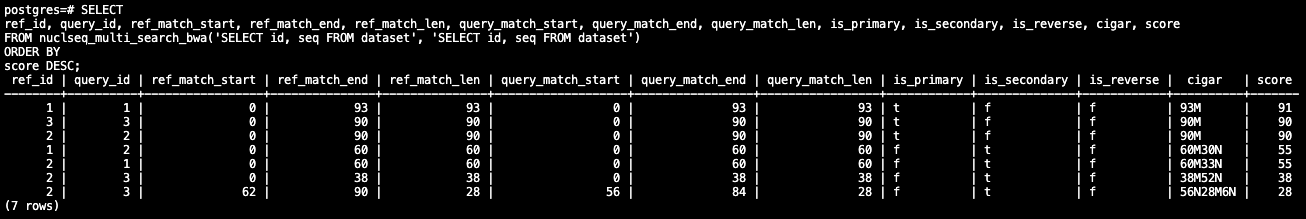
\includegraphics[scale=0.25]{query_screen.png}
  }
\end{frame}
}

\begin{frame}[fragile]
  \frametitle{Execution times}

  \alert{
    Benchmarking using $N \in \{50, 500, 5k, 20k\}$ reference sequences via single query search.
    Query size was 100 and target sequences' sizes 1000.
  }
\end{frame}

\begin{frame}[fragile]
  \frametitle{Execution times}
  \begin{figure}[ht]
    \centering
    \begin{CacheMeCode}{python, custom include command={\input{\robExtAddCachePathAndName{\robExtFinalHash.pgf}}}, set placeholder eval={__LINEWIDTH__}{\lenToCmNoUnit[in]{\linewidth}}}
      import matplotlib.pyplot as plt
      import matplotlib
      import numpy as np
      import json
      matplotlib.use("pgf")
      matplotlib.rcParams.update({
        "font.family": "serif",
        "font.serif": [],
        "text.usetex": True,
      })
      fig, ax = plt.subplots()
      fig.set_size_inches(__LINEWIDTH__, 0.6*__LINEWIDTH__, forward=True)

      cases = { #TODO: move this datapoints
          "single_50": (0.04, 0.02),
          "single_500": (0.15, 0.14),
          "single_5k": (2.01, 1.7),
          "single_20k": (13.49, 11.28),
      }

      width = 0.3
      multiplier = 0
      x = np.arange(len(cases))


      vals_bwa = [program_stats[0] for program_label, program_stats in cases.items()]
      vals_pg = [program_stats[1]-program_stats[0] for program_label, program_stats in cases.items()]

      bottom = [0 for case in cases]
      for (series, color, name) in [
          (vals_bwa, "#ED0020", "BWA time footprint"),
          (vals_pg, "#107AB0", "Postgres overhead"),
      ]:
          ax.bar(x, series, width, bottom=bottom, color=color, label=f"{name}")
          bottom = [bottom[i]+series[i] for i in range(len(bottom))]


      ax.set_xticks(x + width/2)
      ax.set_xticklabels([case.replace('_', '-') for case in cases])
      ax.set_ylabel('Total runtime [s]', fontsize=8)
      #ax.set_yscale("log")
      ax.set_title("Postgre runtime overhead (avg. 50 runs)", fontsize=8)
      ax.legend(loc='upper center', bbox_to_anchor=(0.5, -0.2),
        ncol=2, fancybox=False, shadow=False, prop={'size': 6}, frameon=False)

      print(get_filename_from_extension(".pgf"))
      plt.savefig(get_filename_from_extension(".pgf"), bbox_inches="tight")
    \end{CacheMeCode}
  \end{figure}
\end{frame}

\begin{frame}
  \frametitle{Time/Storage footprint}
  \begin{tabular}{ |c|c| } 
  \hline
  Storage: FASTA file & 19.8MB \\ 
  \hline
  Storage: Compressed FASTA file & 5.9MB \\ 
  \hline
  Storage: PostgreSQL table & 22MB \\ 
  \hline
  \end{tabular} \newline

  \begin{tabular}{ |c|c| } 
  \hline
  RAM BWA & 52MB \\ 
  \hline
  RAM PG & 54MB \\ 
  \hline
  \end{tabular} \newline

  \begin{tcolorbox}[colback=green!5,colframe=green!40!black,title=Memory]
  This comparison is for 20K dataset. Around $10\%$ overhead for PG for storage footprint.
  Minimal $4\%$ overall footprint for memory usage.
  \end{tcolorbox}
  \begin{tcolorbox}[colback=green!5,colframe=green!40!black,title=Time]
  PG is on average $15\%$ slower with a minimal constant penalty of 0.01-0.05s
  \end{tcolorbox}
\end{frame}


\section{Stage III: Custom storage}
\begin{frame}[plain,c]
\begin{center}
\Huge Stage III: Custom storage
\end{center}
\end{frame}

\begin{frame}
  \frametitle{Current plans for Dec-Feb}
  \begin{itemize}
    \item Benchmark for larger dataset up to 10s of GB
    \item Research possible storage implementation via TAMs
    \item Optimized storage along with seet imprint
    \item Incremental index building (with table sequence metrics)
    \item Implement custom alignment algorithm
  \end{itemize}
\end{frame}